% id: 122-13
% book: 개념원리 중학 3-2 · 12 산포도와 표준편차
% section: 중단원 마무리하기 STEP 2 발전 문제
% figure: crop:fig-122-13.png
% answer: $10$
% answer_source: 답지
% variant_level: 0 (원본 전사)
% 이 파일은 build.mjs 가 items.json 에서 만든다. 고칠 때는 items.json 을 고친다.
\smash{\raisebox{1.5mm}{\dmkichul{개념원리 중학 3-2 122쪽 13번 · 꼭나와}}}
다음 표는 수진이가 지난 3월부터 7월까지 도서관에 간 횟수를 조사하여 나타낸 것이다. 이 자료의 평균이 5회이고 분산이 10일 때, $ab$의 값을 구하시오.
\par\smallskip\begin{center}\setlength{\dmfigw}{209.5pt}\ifdim\dmfigw>\linewidth\setlength{\dmfigw}{\linewidth}\fi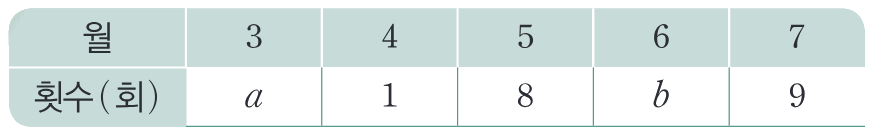
\includegraphics[width=\dmfigw]{figures/fig-122-13.png}\end{center}
